\section{Results and Discussion}

\subsection{Metrics}
%% Introduction to used metrics
Given the fact that in any invoice, there are far fewer fields that are actually classes 1-7 than fields that belong to Other, our data is heavily skewed towards class 0. Thus, the accuracy (percentage error) of the overall model 
is not the most
informative metric, as a good classification on the dominant class would result in a high accuracy
irrespective to performance on the minority classes. Therefore, we computed the precision,
recall, specificity, and the corresponding $F_1$ scores for all classes. 
$F_1$ score is the harmonic mean of precision and recall\cite{powers2011evaluation}, which allows us
to combine precision and recall, which are trade-offs of each other, into one metric. 

\[ \textup{precision} = \frac{\textup{TP}}{\textup{TP}+\textup{FP}} , 
 \textup{recall} = \frac{\textup{TP}}{\textup{TP}+\textup{FN}}\]
\[\textup{specificity} = \frac{\textup{TN}}{\textup{TN}+\textup{FP}},  
 F_1 = 2\cdot \frac{\textup{precision} \cdot \textup{recall}}{\textup{precision} + \textup{recall}} \]

Sometimes, however, it is useful to have a single metric reflecting how well we perform on the minority classes (all classes except ``Other'') in the trade-off space. Therefore, we used another metric -  
the average of $F_1$ scores of all classes 
weighted by the frequency of each class label. To exclude the contribution of the majority class, we excluded the ``Other'' class when calculating the weighted average $F_1$ score. 

\subsection{Regularization Parameter Scaling}
Regularization term is added to Logistic Regression and SVM in Eq.(\ref{eq:logreg}-\ref{eq:SVM}) to reduce overfitting, where $C$ is the regularization parameter that controls the cost of misclassification on the training data \cite{chen2004support}. Fig.\ref{fig:reg} shows the scaling of $C$ with respect to $F_1$ score for both $\ell_1$- and $\ell_2$-regularization.

We can clearly see that the results are less desirable when $C$ is either too small or too large. When $C$ is too small, the cost of misclassification is low on the training data, resulting a overly "soft" hyperplane margin that risks underfitting. When $C$ is too large, the algorithm is forced to explain the input data stricter as the penalty for non-separable points is high, resulting in a model that overfits.

Although $\ell_1$-regularization is computationally more efficient for sparse data, from Fig.\ref{fig:reg} we see that $\ell_2$-regularization in general works better in optimizing the average $F_1$ score we are interested in. Thus, for our model, $\ell_2$-regularization is applied to both Logistic Regionssion and SVM, with $C = 10.72$ for Logistic Regression and $C = 0.58$ for SVM.

\begin{figure}
\centering
\begin{minipage}{.5\linewidth}
  \centering
  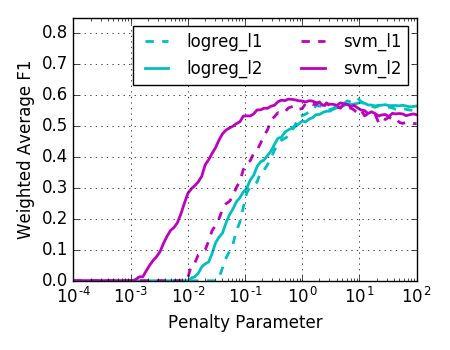
\includegraphics[width=1\linewidth]{reg_K-FOLD}
  \caption{Regularization}
  \label{fig:reg}
\end{minipage}%
\begin{minipage}{.5\linewidth}
  \centering 
  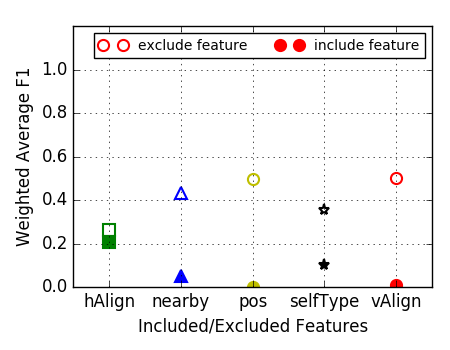
\includegraphics[width=1\linewidth]{incfeatures_K-FOLD_svm_python}
  \caption{Feature Rules Effectiveness}
  \label{fig:fetrule}
\end{minipage}
\end{figure}

\subsection{Feature Selection}

\begin{figure*}[ht]
\centering
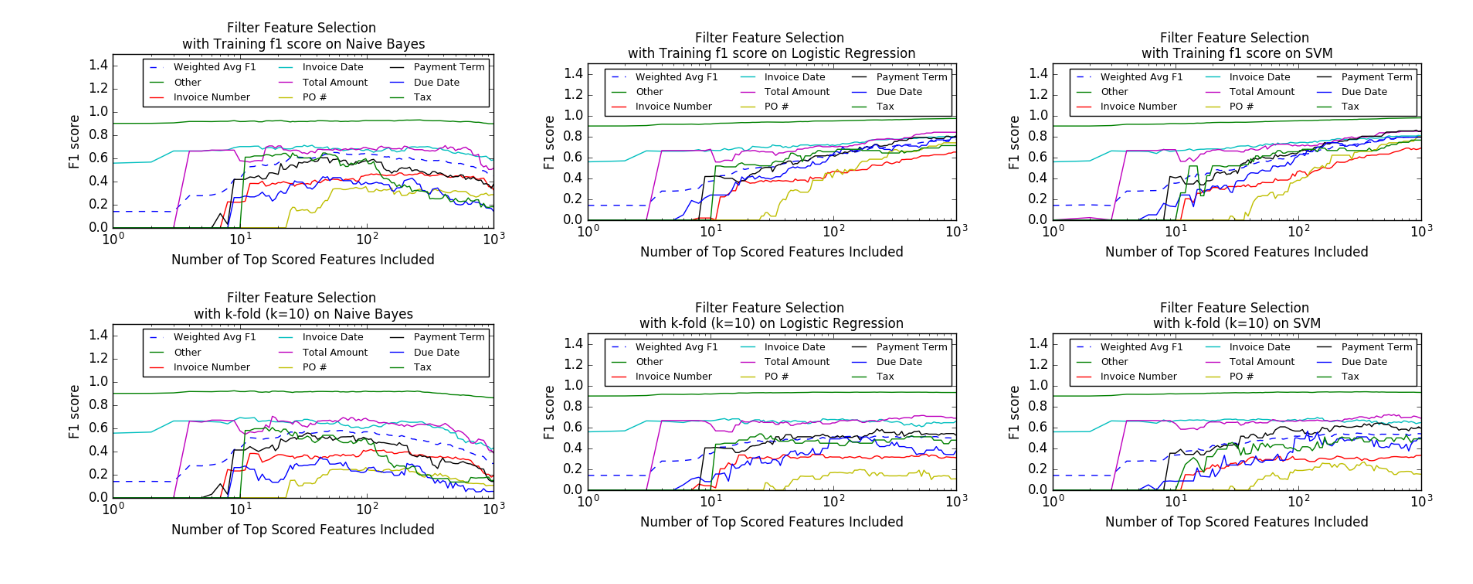
\includegraphics[trim={1cm 0.8cm 0 0}, clip, width=1\linewidth]{filterFS}
\caption{Filter Feature Selection. The solid lines are individual $F_1$ scores for all classes and the dashed line is the weighted average $F_1$ score}
\label{fig:fetsel}
\end{figure*}

%% Feature selection rule effectiveness
Fig.\ref{fig:fetrule} evaluates the effectiveness of each feature selection rule, where solid markers represent weighted average $F_1$ when only that selection rule is included (inclusion set), while hollow markers represent the case when only that rule is excluded (exclusion set). We can easily see that horizontal alignment (hAlign) is the most effective, with best performance in the inclusion set and worst performance in the exclusion set, and is followed by self type (selfTpe), nearby, vertical align (vAlign), and position (pos). It is not a surprise that hAlign is the most effective, as many fields of interests, regardless of the absolute position, are horizontally aligned in a decent number of invoices. On the contrary, while the absolute vertical position was moderately indicative when data size was small, The variety in invoice templates increase dramatically as data set expands, making it harder to derive common properties in layout structure and causing this feature selection rule to be less instructive.

%% Feature selection
Following rule-level analysis, filter feature selection is performed on the individual features to exclude the less indicative ones generated by effective selection rules. First, for every feature, we use the empirical distribution of each feature, $p(x_i)$, and that of each class, $p(y)$, as well as their joint distribution, $p(x_i,y)$, to compute the mutual information MI($x_i, y$) between $x_i$ and $y$, given by the Kullback-Leibler (KL) divergence of the distributions $p(x_i, y)$ and $p(x_i)p(y)$, as
\begin{align*}
\mathrm{MI}(x_i, y) &= \mathrm{KL}(p(x_i, y)\Vert p(x_i)p(y))\\
&=\sum_{x_i\in\{0,1\}}\sum_{y=0}^7p(x_i,y)\log\frac{p(x_i, y)}{p(x_i)p(y)}.
\end{align*}
$\mathrm{MI}(x_i, y)$ thus serves as a score, a large value of which indicates the feature $x_i$ is strongly correlated with the class labels and small otherwise. Therefore, we pick top scored features in our model. To decide how many features 
to include, we sweep the number of top scored features included and use the weighted average $F_1$ score with $k$-fold validation
to threshold desired performance.

Fig.~\ref{fig:fetsel} shows our experimental results for both training $F_1$ score and testing
$F_1$ score computed with $k$-fold cross-validation for three algorithms. For training $F_1$ score,
both SVM and Logistic Regression monotonically increase as more features are included because the
model is overfit. The performance of Naive Bayes, however, first dramatically improves as number of
features increases when feature size is small and then starts to degrade when too many features are
included. This is because Naive Bayes weights probabilities of all features equally and simply
multiply them together. Therefore, the contribution of indicative features to the overall
probability decreases as more features are included, resulting in a downgrade in performance. Similar
but more exaggerated behavior can be observed in testing $F_1$ score for Naive Bayes. Additionally,
Naive Bayes assumes features are independent to each other, which in many cases is not accurate. For
instance, if token 'invoice number' is in nearby region, it is very likely that 'invoice date' and
other header tokens are also in the nearby region. Finally, performance of SVM and Logistic
Regression increases first before reaching constant. The turning point of $F1$ score at 434 number of features is where we threshold amount of features to include, as including more features will 
not improve the performance. 

\subsection{Overall Performance Evaluation}

\begin{table}[!t]
% increase table row spacing, adjust to taste
%\renewcommand{\arraystretch}{1.3}
%if using array.sty, it might be a good idea to tweak the value of
%\extrarowheight as needed to properly center the text within the %cells
\caption{Average Training and Testing Accuracy}
\label{tab:accuracy}
\centering
% Some packages, such as MDW tools, offer better commands for making tables
% than the plain LaTeX2e tabular which is used here.
\begin{tabular}{|c|c|c|}
\hline
 & Training Error (\%) & Testing Error (\%)\\\hline
\begin{tabular}{@{}c@{}}Naive Bayes \\ (9 features)\end{tabular} & 16.17 & 16.43\\\hline
\begin{tabular}{@{}c@{}}Logistic Regression \\ (249 features)\end{tabular} & 10.95 & 14.53\\\hline
\begin{tabular}{@{}c@{}}SVM \\ (157 features)\end{tabular} & 8.81 & 13.99\\\hline
\end{tabular}
\end{table}

\begin{figure*}[ht]
\centering
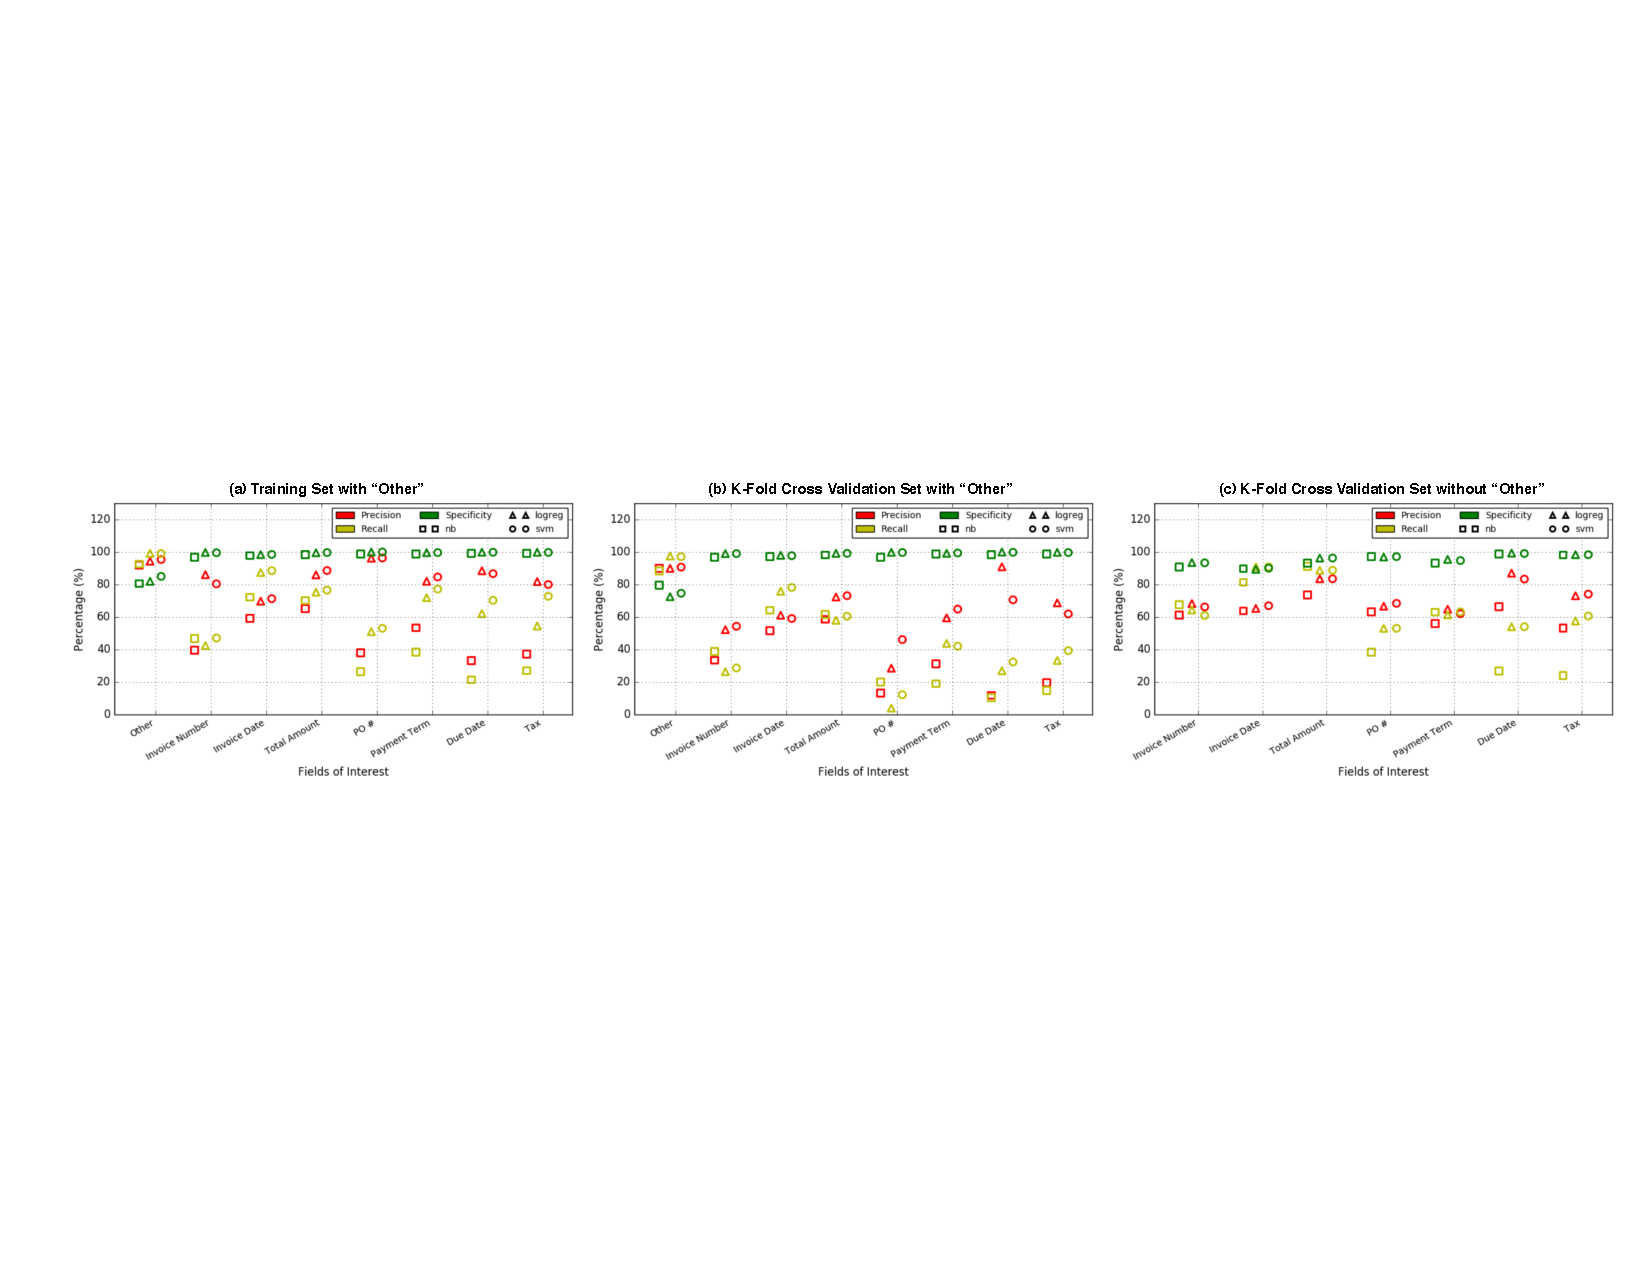
\includegraphics[width=1\linewidth, trim={1cm 8cm 0.3cm 8cm}, clip, ]{model_all.pdf}
\caption{Classifier Overall Performance, measured by Precision, Recall, and Specificity}
\label{fig:model}
\end{figure*}

Table \ref{tab:accuracy} shows the best $k$-fold cross validation accuracy achieved and training accuracy for three algorithms with corresponding number of top scored features.  There is only slight overfitting in Logistic Regression and SVM due to application of regularization and overall accuracy is promising.

Fig. \ref{fig:model} shows the precision, recall, and specificity of all classes and three algorithms on training and test data computed with $k$-fold cross validation. The trade-off between precision and recall can be found in most classes. Fig. \ref{fig:model}(a) shows that our models performs well across all classes on the training data. However, comparison between \ref{fig:model}(a) and (b) shows that our algorithms have a high variance for Invoice Number and PO \#, which suggests overfitting. These fields are especially prone to overfitting because their bag of features vary hugely and we have a especially small quantity of PO \# tokens.

It can be seen from Fig. \ref{fig:model}(a) \& (b) that for almost all classes,  Naive Bayes has a worse performance than Logistic Regression and SVM in terms of both precision and recall.  We believe that this is largely due to the aforementioned fact that the Naive Bayes model makes the assumption that all features are conditionally independent given the class labels, which likely does not hold in this classification context. Logistic Regression and SVM have similar precision in all fields of interest but \textit{PO \#}, \textit{Due Date}, and \textit{Tax}, with SVM performing slightly better. SVM outperforms Logistic Regression for \textit{PO \#}, whereas Logistic Regression has better performance for \textit{Due Date} and \textit{Tax}. One major difference between these fields is that fields that are \textit{PO \#}'s can vary largely in terms of its type and its position in the invoice file, whereas \textit{Due Date} and \textit{Tax} are generally of the same type (date and money, respectively), and can be identified by self type more easily.  This suggests that SVM is better than Logistic Regression at extracting the most useful features among all when making a prediction.

Another important observation is that except \textit{Other} (class label 0), all fields of interest suffer from low recall regardless of which algorithm is used, but have very high specificity, whereas the \textit{Other} field has very high recall but low specificity. This indicates that it is very easy for our learning algorithms to mis-classify fields like \textit{Invoice Number}, \textit{Invoice Date}, etc.\ (class labels 1-7) as \textit{Other},  while there are very few instances where \textit{Other} is classified as the rest of the fields. The reason is that the \textit{Other} field actually contains all different type of fields that are unlabeled in our data, which results in a highly skewed class distribution and leads to a very high tendency for our algorithm to predict a field to be \textit{Other}. This argument can be further corroborated by Fig. \ref{fig:model}(c), which is the same plot but without the \textit{Other} field. It can easily be seen that the performance across all fields of interest dramatically increases, especially for precision and recall. In other words, our algorithm can reliably tell whether a field belongs to one class or another among class labels 1-7, but because of the presence of large amount of tokens belonging to \textit{Other} and \textit{Other} exhibits large range of feature characteristics, our performance suffers from the high rate of misclassifying 1-7 as 0. We believe the issue can be alleviated when more training data are available and more type of fields of interest are labeled in our training data.

